% Foliensatz: "AFu-Kurs nach DJ4UF" von DK0TU, Amateurfunkgruppe der TU Berlin
% Lizenz: CC BY-NC-SA 3.0 de (http://creativecommons.org/licenses/by-nc-sa/3.0/de/)
% Autoren: Lars Weiler <dc4lw@darc.de>
% Korrekturen: Sebastian Lange <dl7bst@dk0tu.de>, DL7XJ

preamble.dk0tu.tex
\subtitle{Technik A14: \\
           Digitaltechnik \\[2em]}
\date{Stand 22.02.2016}
 \begin{document}

\begin{frame}
    \titlepage
    \vfill
    \begin{center}
        \ccbyncsaeu\\
        {\tiny This work is licensed under the \em{Creative Commons Attribution-NonCommercial-ShareAlike 3.0 License}.}\\[0.5ex]
         \tiny Amateurfunkgruppe der Technische Universität Berlin (AfuTUB), DKØTU
         %\includegraphics[scale=0.5]{img/DK0TU_Logo.pdf}
    \end{center}
\end{frame}


\begin{frame}{Digitaltechnik}
  Die Digitaltechnik kennt nur zwei Zustände:
  \begin{description}
    \item[0] LOW
    \item[1] HIGH
  \end{description}
  Zwischenwerte, wie in der Analogtechnik, sind nicht vorhanden.\\[2em]
  In der Realität ist es eine Definitionssache, ab welcher Spannung ein Signal als LOW oder HIGH angesehen wird.
\end{frame}


\section{Transistor als Schalter}


\begin{frame}{Transistor als Schalter}
  \begin{columns}
    \column{.5\textwidth}
      \includegraphics[width=\textwidth,height=.8\textheight,keepaspectratio]{a14/td401_simplified.png}\\
      {\tiny TD401 \hyperlink{refs}{\cite{bna}}}\\
    \column{.45\textwidth}
      \pause
      \begin{itemize}
        \item Transistor in Emitterschaltung
        \item Liegt am Eingang keine Spannung an, ist die Ausgangsspannung maximal
        \item Liegt am Eingang eine hohe Spannung an, wird die Ausgangsspannung minimal
        \item $\rightarrow$ \textbf{Inverter}
          \pause
        \item Es gibt in der Prüfung nur zwei Transistor-Logik-Schaltungen
        \item Zuerst ein Blick auf die Logikgatter
      \end{itemize}
  \end{columns}
\end{frame}

\subsection{NOT}

\begin{frame}{NOT}
  \begin{columns}
    \column[c]{.4\textwidth}
    \includegraphics[width=\textwidth,height=.2\textheight,keepaspectratio]{a14/NOT_IEC.pdf}\\
    {\small Schaltsymbol IEC}\\
    \includegraphics[width=\textwidth,height=.2\textheight,keepaspectratio]{a14/NOT_DIN.pdf}\\
    {\small Schaltsymbol DIN}\\
    \includegraphics[width=\textwidth,height=.2\textheight,keepaspectratio]{a14/NOT_ANSI.pdf}\\
    {\small Schaltsymbol ANSI}
    \column{.55\textwidth}
    \begin{block}{Wahrheitstabelle}
      \begin{tabular}{c|c}
        \textbf{INPUT} & \textbf{OUTPUT} \\
        \textbf{A} & \textbf{NOT A} \\ \hline
        0 & 1 \\
        1 & 0 \\
      \end{tabular}
    \end{block}
  \end{columns}
\end{frame}

\subsection{AND}
\begin{frame}{AND}
  \begin{columns}
    \column[c]{.4\textwidth}
    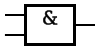
\includegraphics[width=\textwidth,height=.2\textheight,keepaspectratio]{a14/AND_IEC.pdf}\\
    {\small Schaltsymbol IEC}\\
    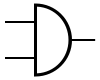
\includegraphics[width=\textwidth,height=.2\textheight,keepaspectratio]{a14/AND_DIN.pdf}\\
    {\small Schaltsymbol DIN}\\
    \includegraphics[width=\textwidth,height=.2\textheight,keepaspectratio]{a14/AND_ANSI.pdf}\\
    {\small Schaltsymbol ANSI}
    \column{.55\textwidth}
    \begin{block}{Wahrheitstabelle}
      \begin{tabular}{cc|c}
        \multicolumn{2}{c|}{\textbf{INPUT}} & \textbf{OUTPUT} \\
        \textbf{A} & \textbf{B} & \textbf{A AND B} \\ \hline
        0 & 0 & 0 \\
        0 & 1 & 0 \\
        1 & 0 & 0 \\
        1 & 1 & 1 \\
      \end{tabular}
    \end{block}
  \end{columns}
\end{frame}

\subsection{NAND}

\begin{frame}{NAND}
  \begin{columns}
    \column[c]{.4\textwidth}
    \includegraphics[width=\textwidth,height=.2\textheight,keepaspectratio]{a14/NAND_IEC.pdf}\\
    {\small Schaltsymbol IEC}\\
    \includegraphics[width=\textwidth,height=.2\textheight,keepaspectratio]{a14/NAND_DIN.pdf}\\
    {\small Schaltsymbol DIN}\\
    \includegraphics[width=\textwidth,height=.2\textheight,keepaspectratio]{a14/NAND_ANSI.pdf}\\
    {\small Schaltsymbol ANSI}
    \column{.55\textwidth}
    \begin{block}{Wahrheitstabelle}
      \begin{tabular}{cc|c}
        \multicolumn{2}{c|}{\textbf{INPUT}} & \textbf{OUTPUT} \\
        \textbf{A} & \textbf{B} & \textbf{A NAND B} \\ \hline
        0 & 0 & 1 \\
        0 & 1 & 1 \\
        1 & 0 & 1 \\
        1 & 1 & 0 \\
      \end{tabular}
    \end{block}
  \end{columns}
\end{frame}

\subsection{OR}

\begin{frame}{OR}
  \begin{columns}
    \column[c]{.4\textwidth}
    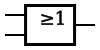
\includegraphics[width=\textwidth,height=.2\textheight,keepaspectratio]{a14/OR_IEC.pdf}\\
    {\small Schaltsymbol IEC}\\
    \includegraphics[width=\textwidth,height=.2\textheight,keepaspectratio]{a14/OR_DIN.pdf}\\
    {\small Schaltsymbol DIN}\\
    \includegraphics[width=\textwidth,height=.2\textheight,keepaspectratio]{a14/OR_ANSI.pdf}\\
    {\small Schaltsymbol ANSI}
    \column{.55\textwidth}
    \begin{block}{Wahrheitstabelle}
      \begin{tabular}{cc|c}
        \multicolumn{2}{c|}{\textbf{INPUT}} & \textbf{OUTPUT} \\
        \textbf{A} & \textbf{B} & \textbf{A OR B} \\ \hline
        0 & 0 & 0 \\
        0 & 1 & 1 \\
        1 & 0 & 1 \\
        1 & 1 & 1 \\
      \end{tabular}
    \end{block}
  \end{columns}
\end{frame}

\subsection{NOR}

\begin{frame}{NOR}
  \begin{columns}
    \column[c]{.4\textwidth}
    \includegraphics[width=\textwidth,height=.2\textheight,keepaspectratio]{a14/NOR_IEC.pdf}\\
    {\small Schaltsymbol IEC}\\
    \includegraphics[width=\textwidth,height=.2\textheight,keepaspectratio]{a14/NOR_DIN.pdf}\\
    {\small Schaltsymbol DIN}\\
    \includegraphics[width=\textwidth,height=.2\textheight,keepaspectratio]{a14/NOR_ANSI.pdf}\\
    {\small Schaltsymbol ANSI}
    \column{.55\textwidth}
    \begin{block}{Wahrheitstabelle}
      \begin{tabular}{cc|c}
        \multicolumn{2}{c|}{\textbf{INPUT}} & \textbf{OUTPUT} \\
        \textbf{A} & \textbf{B} & \textbf{A NOR B} \\ \hline
        0 & 0 & 1 \\
        0 & 1 & 0 \\
        1 & 0 & 0 \\
        1 & 1 & 0 \\
      \end{tabular}
    \end{block}
  \end{columns}
\end{frame}

\subsection{XOR}

\begin{frame}{XOR}
  \begin{columns}
    \column[c]{.4\textwidth}
    \includegraphics[width=\textwidth,height=.2\textheight,keepaspectratio]{a14/XOR_IEC.pdf}\\
    {\small Schaltsymbol IEC}\\
    \includegraphics[width=\textwidth,height=.2\textheight,keepaspectratio]{a14/XOR_DIN.pdf}\\
    {\small Schaltsymbol DIN}\\
    \includegraphics[width=\textwidth,height=.2\textheight,keepaspectratio]{a14/XOR_ANSI.pdf}\\
    {\small Schaltsymbol ANSI}
    \column{.55\textwidth}
    \begin{block}{Wahrheitstabelle}
      \begin{tabular}{cc|c}
        \multicolumn{2}{c|}{\textbf{INPUT}} & \textbf{OUTPUT} \\
        \textbf{A} & \textbf{B} & \textbf{A XOR B} \\ \hline
        0 & 0 & 0 \\
        0 & 1 & 1 \\
        1 & 0 & 1 \\
        1 & 1 & 0 \\
      \end{tabular}
    \end{block}
  \end{columns}
\end{frame}

\subsection{Fragen}

\begin{frame}
  \begin{tabular}{l||p{.8\textwidth}}\hline
    \textbf{TC703} & \textbf{Wie heißen die Grundbausteine in der Digitaltechnik} \\ \hline\hline
    A & (+)-Gatter (UND), (-)-Gatter (OR), NICHT-(+)-Gatter (NUND), NICHT-(-)-Gatter (NODER). \\ \hline
    B & UND-Gatter (UNG), ODER-Gatter (ORG), NICHT-UND-Gatter (NUNG), NICHT-ODER-Gatter (NORG). \\ \hline
    C & UND-Glied (UND), ODER-Glied (ODER), NICHT-UND-Glied (NUND), NICHT-ODER-Glied (NODER). \\ \hline
    D \only<2>\checkmark & UND-Glied (AND), ODER-Glied (OR), NICHT-UND-Glied (NAND), NICHT-ODER-Glied (NOR). \\ \hline
  \end{tabular}
\end{frame}

\begin{frame}
  \begin{scriptsize}
    \begin{tabular}{l||p{.8\textwidth}}\hline
      \textbf{TC705} & \textbf{Welche logische Grundschaltung stellt die folgende Transistorschaltung dar und wie arbeitet sie?}

      \includegraphics[width=.5\textwidth,height=.3\textheight,keepaspectratio]{a14/tc705.png}\\ \hline\hline
      A & Die Schaltung stellt ein OR-Gatter dar. Der Ausgang Z führt dann Nullpotential, wenn die Eingänge A und B mit der Betriebsspannung verbunden sind. In allen anderen Fällen führt der Ausgang Z die Betriebsspannung. \\ \hline
      B & Die Schaltung stellt ein NOR-Gatter [negiertes ODER-Gatter] dar. Der Ausgang Z führt dann die Betriebsspannung, wenn keiner der beiden Eingänge A oder B mit der Betriebsspannung verbunden ist. In allen anderen Fällen führt der Ausgang Z Nullpotential. \\ \hline
      C \only<2>\checkmark & Die Schaltung stellt ein NAND-Gatter [negiertes UND-Gatter] dar. Der Ausgang Z führt dann Nullpotential, wenn die Eingänge A und B mit der Betriebsspannung verbunden sind. In allen anderen Fällen führt der Ausgang Z die Betriebsspannung. \\ \hline
      D & Die Schaltung stellt ein AND-Gatter dar. Der Ausgang Z führt dann Betriebsspannung, wenn die Eingänge A und B mit der Betriebsspannung verbunden sind. In allen anderen Fällen führt der Ausgang Z Nullpotential. \\ \hline
    \end{tabular}
  \end{scriptsize}
\end{frame}

\begin{frame}
  \begin{scriptsize}
    \begin{tabular}{l||p{.8\textwidth}}\hline
      \textbf{TC706} & \textbf{Welche logische Grundschaltung stellt die folgende Transistorschaltung dar und wie arbeitet sie?}

      \includegraphics[width=.5\textwidth,height=.3\textheight,keepaspectratio]{a14/tc706.png}\\ \hline\hline
      A \only<2>\checkmark & Die Schaltung stellt ein NOR-Gatter [negiertes ODER-Gatter] dar. Der Ausgang Z führt dann die Betriebsspannung, wenn beide Eingänge A und B Nullpotential führen bzw. offen sind. In allen anderen Fällen führt der Ausgang Z Nullpotential. \\ \hline
      B & Die Schaltung stellt ein NAND-Gatter [negiertes UND-Gatter] dar. Der Ausgang Z führt dann Nullpotential, wenn die Eingänge A und B mit der Betriebsspannung verbunden sind. In allen anderen Fällen führt der Ausgang Z die Betriebsspannung. \\ \hline
      C & Die Schaltung stellt ein OR-Gatter dar. Der Ausgang Z führt dann Betriebsspannung, wenn die Eingänge A und B mit der Betriebsspannung verbunden sind. In allen anderen Fällen führt der Ausgang Z die Nullpotential. \\ \hline
      D & Die Schaltung stellt ein AND-Gatter dar. Der Ausgang Z führt dann Nullpotential, wenn die Eingänge A und B mit der Betriebsspannung verbunden sind. In allen anderen Fällen führt der Ausgang Z Betriebsspannung. \\ \hline
    \end{tabular}
  \end{scriptsize}
\end{frame}

\section{Zeit"-ablauf"-diagramme}
\begin{frame}{Zeitablaufdiagramme}
  \begin{columns}
    \column[c]{.45\textwidth}
    \includegraphics[width=\textwidth,height=.8\textheight,keepaspectratio]{a14/tc707.png}\\
    {\tiny TC707--TC709 \hyperlink{refs}{\cite{bna}}}
    \column[c]{.5\textwidth}
    \begin{itemize}
      \item zur Überprüfung digitaler Schaltungen
      \item an die Eingänge werden wechselnde Signale angelegt
      \item die Beobachtung des Ausgangs mit einem Speicheroszilloskop ergibt Rückschlüsse auf die verwendete Schaltung
    \end{itemize}
    \pause
    \begin{description}
      \item[$x_1\rightarrow$] \only<3>{OR}
      \item[$x_2\rightarrow$] \only<3>{AND}
      \item[$x_3\rightarrow$] \only<3>{XOR}
      \item[$x_4\rightarrow$] \only<3>{NOR}
    \end{description}
  \end{columns}
\end{frame}

\section{Logik"-schaltungen}
\begin{frame}{Logikschaltungen}
  \begin{columns}
    \column[c]{.45\textwidth}
    \includegraphics[width=\textwidth,height=.8\textheight,keepaspectratio]{a14/tc704.png}\\
    {\tiny TC704 \hyperlink{refs}{\cite{bna}}}
    \column[c]{.5\textwidth}
    \begin{itemize}
      \item Zusammenschaltung mehrerer Logikgatter
      \item Komplexe Aufgaben können bewältigt werden
      \item ``Programmieren in Hardware''
      \item Beispiele sind Schaltungen für Rechenoperationen, Flipflops oder Multiplexer
      \item Daraus lassen sich wiederum Datenspeicher, Zähler oder ganze Mikroprozessoren aufbauen
      \item \emph{Beispiel: \href{https://media.ccc.de/v/gpn14_-_5862_-__-_medientheater_-_201406211600_-_zuse_z22_-_lorenz_hanewinkel}{$\Rightarrow$ Lorenz Hanewinkel über die Konstruktion der Z22}}
    \end{itemize}
  \end{columns}
\end{frame}

\begin{frame}{Beispiel: R-S-Flipflop}
  \begin{columns}
    \column{.48\textwidth}
    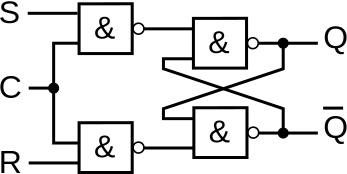
\includegraphics[width=\textwidth,height=.8\textheight,keepaspectratio]{a14/ISO-RS-FF-NAND-with-clock.png}\\
    {\tiny Logik-Schaltung eines getakteten RS-Flipflops aus vier NAND-Gattern \hyperlink{refs}{\cite{wp}}}
    \column{.48\textwidth}
    \includegraphics[width=\textwidth,height=.8\textheight,keepaspectratio]{a14/SR_latch_impulse_diagram.png}\\
    {\tiny Impulsdiagramm (SR-Latch) \hyperlink{refs}{\cite{wp}}}
  \end{columns}
\end{frame}


\begin{frame}
  \begin{tabular}{l||p{.8\textwidth}}\hline
    \textbf{TC704} & \textbf{Welche der Aussagen trifft für diese Schaltung zu?}

    \includegraphics[width=.6\textwidth,height=.6\textheight,keepaspectratio]{a14/tc704.png}\\ \hline\hline
    A & X=1 und Y=0 \\ \hline
    B \only<2>\checkmark & X=0 und Y=0 \\ \hline
    C & X=1 und Y=1 \\ \hline
    D & X=0 und Y=1 \\ \hline
  \end{tabular}
\end{frame}

\section{Pegel"-anpassung}
\begin{frame}{Pegelanpassung}
  \begin{itemize}
    \item nicht alle ICs oder Schaltungen liefern 0 und +5V
    \item durch entsprechende Pegelwandler können die Pegel normiert werden
    \item \emph{wird in der Prüfung nicht gefragt, aber nützliches Wissen, wenn der 5V-Ausgang des Arduino den 3,3V-GPIO am Raspberry Pi brät\ldots}
  \end{itemize}
\end{frame}

\begin{frame}
  \begin{tabular}{l||p{.8\textwidth}}\hline
    \textbf{TC710} & \textbf{In welchem Versorgungsspannungsbereich können CMOS-ICs betrieben werden?} \\ \hline\hline
    A \only<2>\checkmark & $+3V$ bis $+15V$ \\ \hline
    B & $+2,5V$ bis $+5,5V$ \\ \hline
    C & $\pm2,5V$ bis $\pm5,5V$ \\ \hline
    D & $\pm5V$ \\ \hline
  \end{tabular}
\end{frame}

\section{Zahlensysteme}

\subsection{Dual}
\begin{frame}{Dualzahlen}
  \begin{exampleblock}{}
    {\Large``There are only 10 types of people in the world:\\
    those who understand binary, and those who don't.''}\\[1em]
    \hspace*\fill{\small--- Mathematical joke}
  \end{exampleblock}
\end{frame}

\begin{frame}{Dualzahlen}
  \begin{columns}
    \column{.5\textwidth}
    \begin{tabular}{r|c|r}
      \textbf{Binär} & \textbf{Potenz} & \textbf{Dezimal} \\ \hline
      0 & $0$ & 0 \\
      1 & $2^0$ & 1 \\
      10 & $2^1$ & 2 \\
      11 & $2^1+2^0$ & 3 \\
      100 & $2^2$ & 4 \\
      101 & $2^2+2^0$ & 5 \\
      110 & $2^2+2^1$ & 6 \\
      111 & $2^2+2^1+2^0$ & 7 \\
    \end{tabular}
    \column{.5\textwidth}
    \begin{tabular}{r|c|r}
      \textbf{Binär} & \textbf{Potenz} & \textbf{Dezimal} \\ \hline
      0 & $0$ & 0 \\
      1 & $2^0$ & 1 \\
      10 & $2^1$ & 2 \\
      100 & $2^2$ & 4 \\
      1000 & $2^3$ & 8 \\
      10000 & $2^4$ & 16 \\
      100000 & $2^5$ & 32 \\
      1000000 & $2^6$ & 64 \\
      10000000 & $2^7$ & 128 \\
      100000000 & $2^8$ & 256 \\
      1000000000 & $2^9$ & 512 \\
      10000000000 & $2^{10}$ & 1024 \\
    \end{tabular}
  \end{columns}
\end{frame}

\begin{frame}
  \begin{tabular}{l||p{.8\textwidth}}\hline
    \textbf{TC722} & \textbf{Welche dezimalen Werte haben die Stellen der Dualzahl 111111 von links nach rechts?} \\ \hline\hline
    A & 1, 2, 4, 8, 16, 32 \\ \hline
    B \only<2>\checkmark & 32, 16, 8, 4, 2, 1 \\ \hline
    C & 65536, 256, 16, 4, 2, 1 \\ \hline
    D & 100000, 10000, 1000, 100, 10, 1 \\ \hline
  \end{tabular}
\end{frame}

\begin{frame}
  \begin{tabular}{l||p{.8\textwidth}}\hline
    \textbf{TC720} & \textbf{Berechnen Sie den dezimalen Wert der 8-Bit-Dualzahl 10001110. Die Dezimalzahl lautet} \\ \hline\hline
    A & 78. \\ \hline
    B \only<2>\checkmark & 142. \\ \hline
    C & 156. \\ \hline
    D & 248. \\ \hline
  \end{tabular}
\end{frame}


\subsection{Hexadezimal}
\begin{frame}{Hexadezimalzahlen}
  \begin{columns}
    \column{.5\textwidth}
    \begin{tabular}{r|r}
      \textbf{Hexadezimal} & \textbf{Dezimal} \\ \hline
      0 & 0 \\
      1 & 1 \\
      2 & 2 \\
      $\vdots$ & $\vdots$ \\
      9 & 9 \\
      A & 10 \\
      B & 11 \\
      C & 12 \\
      D & 13 \\
      E & 14 \\
      F & 15 \\
    \end{tabular}
    \column{.5\textwidth}
    \begin{tabular}{r|r}
      \textbf{Hexadezimal} & \textbf{Dezimal} \\ \hline
      10 & 16 \\
      11 & 17 \\
      $\vdots$ & $\vdots$ \\
      1F & 31 \\
      20 & 32 \\
      21 & 33 \\
      $\vdots$ & $\vdots$ \\
      FE & 254 \\
      FF & 255 \\
    \end{tabular}
  \end{columns}
\end{frame}

\begin{frame}
  \begin{tabular}{l||p{.8\textwidth}}\hline
    \textbf{TC721} & \textbf{Wie lautet der dezimale Wert der zweistelligen Hexadezimalzahl 1A? Die Dezimalzahl lautet} \\ \hline\hline
    A & 16. \\ \hline
    B & 11. \\ \hline
    C \only<2>\checkmark & 26. \\ \hline
    D & 160. \\ \hline
  \end{tabular}
\end{frame}


\renewcommand{\refname}{Referenzen}

\hypertarget{refs}{}
\textcolor{white}{} \\ %\vspace{} geht nicht
\Large Referenzen/Links
\footnotesize

\begin{thebibliography}{}
  \bibitem{darc}  DARC Online-Lehrgang Lektion A14:\\
    \url{https://www.darc.de/der-club/referate/ajw/lehrgang-ta/a14/}
  \bibitem{wm} 	Wikimedia:\\
    \href{https://commons.wikimedia.org/wiki/Logic_gates_unified_symbols}{Logic Gates Unified Symbols, Public Domain}\\
  \bibitem{wp}    Wikipedia - Die freie Enzyklopädie:\\
    \href{https://de.wikipedia.org/wiki/Flipflop}{Flipflop}\\
  \bibitem{bna}   Fragenkatalog Bundesnetzagentur Technik Klasse A:\\
    \url{https://www.bundesnetzagentur.de/SharedDocs/Downloads/DE/Sachgebiete/Telekommunikation/Unternehmen_Institutionen/Frequenzen/Amateurfunk/Fragenkatalog/TechnikFragenkatalogKlasseAf252rId9014pdf.pdf?__blob=publicationFile&v=3}
\end{thebibliography}

% Hier könnte noch eine Kontaktfolie stehen

\end{document}

